\section{How Machines Learn}
\begin{frame}{}
    \LARGE Part 2: \textbf{How Machines Learn}
\end{frame}

\begin{frame}{Two Ways to Make a Computer Do Something}
    \textbf{Machine Learning} gives computers the ability to learn from data, without being explicitly programmed.
    \vspace{1em}

    \begin{columns}
        \begin{column}{0.48\textwidth}
            \centering
            \includegraphics[width=\linewidth,height=0.42\textheight,keepaspectratio]{images/traditional.png}

            \vspace{0.6em}
            \textit{The traditional approach} \\
            \textbf{A person writes the rules}
        \end{column}
        \begin{column}{0.48\textwidth}
            \centering
            \includegraphics[width=\linewidth,height=0.42\textheight,keepaspectratio]{images/ml.png}

            \vspace{0.6em}
            \textit{The Machine Learning approach} \\
            \textbf{The computer finds the rules from examples}
        \end{column}
    \end{columns}
\end{frame}

\begin{frame}{Example: Catching Spam}
    \begin{columns}[T]
        \begin{column}{0.48\textwidth}
            \begin{tcolorbox}[colback=red!5, colframe=red!50, title=\textbf{Writing rules by hand}, equal height group=spam]
                \small
                \begin{itemize}
                    \setlength\itemsep{0.3em}
                    \item If the email says ``free money'' $\rightarrow$ spam
                    \item If it says ``you won a prize'' $\rightarrow$ spam
                    \item If it has 5 exclamation marks $\rightarrow$ spam
                    \item \ldots and hundreds more
                \end{itemize}
                \vspace{0.4em}
                \textbf{Problem:} spammers write ``fr3e m0ney'' and every rule breaks.
            \end{tcolorbox}
        \end{column}
        \begin{column}{0.48\textwidth}
            \begin{tcolorbox}[colback=blue!5, colframe=blue!50, title=\textbf{Learning from examples}, equal height group=spam]
                \small
                \begin{itemize}
                    \setlength\itemsep{0.3em}
                    \item Collect thousands of emails
                    \item People mark each one: \textit{spam} or \textit{not spam}
                    \item The computer finds the patterns that separate the two
                \end{itemize}
                \vspace{0.4em}
                \textbf{Benefit:} when spammers change, we add new examples and it learns again.
            \end{tcolorbox}
        \end{column}
    \end{columns}
\end{frame}

\begin{frame}{The Recipe: Data, Training, Model}
    \centering
    \begin{tikzpicture}[
        box/.style={rectangle, draw, rounded corners, thick, minimum height=1.2cm,
                    text width=2.5cm, align=center, font=\small\bfseries},
        line/.style={draw, -{Latex[length=3mm]}, thick}]
        \node[box, fill=KAUSTblue!10] (data) at (0,0) {Data\\{\normalfont\scriptsize many examples}};
        \node[box, fill=orange!15] (train) at (4.2,0) {Training\\{\normalfont\scriptsize find the patterns}};
        \node[box, fill=KAUSTcyan!15] (model) at (8.4,0) {Model\\{\normalfont\scriptsize what was learned}};
        \node[box, fill=white] (new) at (4.2,-2.1) {A new email\\{\normalfont\scriptsize never seen before}};
        \node[box, fill=green!12] (pred) at (11.9,-2.1) {Prediction\\{\normalfont\scriptsize ``this is spam''}};
        \path[line] (data) -- (train);
        \path[line] (train) -- (model);
        \path[line] (new) -| (model);
        \path[line] (model) -| (pred);
    \end{tikzpicture}

    \vspace{1em}
    \raggedright
    \begin{itemize}
        \setlength\itemsep{0.3em}
        \item \textbf{Data}: the examples we learn from.
        \item \textbf{Training}: the computer adjusts itself until its answers match the examples.
        \item \textbf{Model}: the result of training --- a program that can answer new cases.
    \end{itemize}
\end{frame}

\begin{frame}{Three Ways of Learning}
    \centering
    \renewcommand{\arraystretch}{1.6}
    \begin{tabular}{@{} >{\raggedright\arraybackslash}p{0.22\textwidth}
                        >{\raggedright\arraybackslash}p{0.33\textwidth}
                        >{\raggedright\arraybackslash}p{0.35\textwidth} @{}}
        \toprule
        \textbf{Type} & \textbf{The idea} & \textbf{Like\ldots} \\
        \midrule
        \textbf{Supervised} & Learn from examples that come with the right answer
            & A student with an answer key \\
        \textbf{Unsupervised} & Find patterns in data that has no answers
            & Sorting a box of mixed buttons into piles \\
        \textbf{Reinforcement} & Learn by trying, and getting rewards or penalties
            & Learning to ride a bicycle \\
        \bottomrule
    \end{tabular}
\end{frame}

\begin{frame}{Supervised Learning: Learning with Answers}
    \textit{Every example comes with the correct answer. Two common kinds of question:}
    \vspace{0.6em}

    \begin{columns}[T]
        \begin{column}{0.48\textwidth}
        \centering
            \textbf{``How much?''} \\
            \textit{Predict a number} \\
            \vspace{0.5em}
            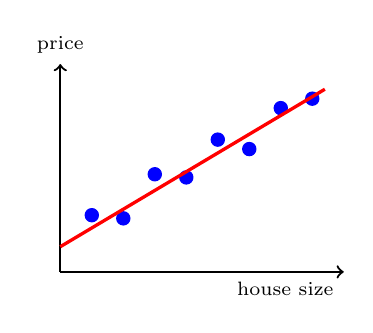
\begin{tikzpicture}[scale=0.8]
                \draw[->, thick] (0,0) -- (4.5,0) node[below left] {\scriptsize house size};
                \draw[->, thick] (0,0) -- (0,3.3) node[above] {\scriptsize price};
                \foreach \x/\d in {0.5/0.2,1/-0.15,1.5/0.25,2/-0.1,2.5/0.2,3/-0.25,3.5/0.1,4/-0.05}
                    \filldraw [blue] (\x, 0.6*\x + 0.4 + \d) circle (3pt);
                \draw [red, very thick] (0,0.4) -- (4.2,2.9);
            \end{tikzpicture}

            \small House prices, temperature, delivery time
        \end{column}
        \begin{column}{0.48\textwidth}
        \centering
            \textbf{``Which one?''} \\
            \textit{Predict a category} \\
            \vspace{0.5em}
            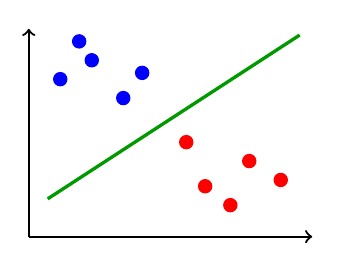
\begin{tikzpicture}[scale=0.8]
                \draw[->, thick] (0,0) -- (4.5,0);
                \draw[->, thick] (0,0) -- (0,3.3);
                \foreach \p in {(0.5,2.5), (1,2.8), (1.5,2.2), (0.8,3.1), (1.8,2.6)}
                    \filldraw [blue] \p circle (3pt);
                \foreach \p in {(2.8,0.8), (3.5,1.2), (3.2,0.5), (4,0.9), (2.5,1.5)}
                    \filldraw [red] \p circle (3pt);
                \draw [green!60!black, very thick] (0.3,0.6) -- (4.3,3.2);
            \end{tikzpicture}

            \small Spam or not, cat or dog, healthy or sick
        \end{column}
    \end{columns}
\end{frame}

\begin{frame}{Unsupervised Learning: Finding Groups}
    \begin{columns}[c]
        \begin{column}{0.45\textwidth}
            \centering
            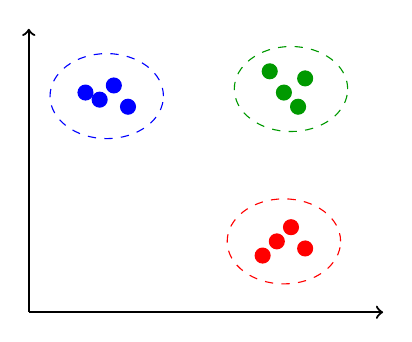
\begin{tikzpicture}[scale=0.9]
                \draw[->, thick] (0,0) -- (5,0);
                \draw[->, thick] (0,0) -- (0,4);
                \foreach \p in {(1,3), (1.2,3.2), (0.8,3.1), (1.4,2.9)}
                    \filldraw [blue] \p circle (3pt);
                \draw [blue, dashed] (1.1,3.05) ellipse (0.8cm and 0.6cm);
                \foreach \p in {(3.5,1), (3.7,1.2), (3.3,0.8), (3.9,0.9)}
                    \filldraw [red] \p circle (3pt);
                \draw [red, dashed] (3.6,1) ellipse (0.8cm and 0.6cm);
                \foreach \p in {(3.6,3.1), (3.9,3.3), (3.4,3.4), (3.8,2.9)}
                    \filldraw [green!60!black] \p circle (3pt);
                \draw [green!60!black, dashed] (3.7,3.15) ellipse (0.8cm and 0.6cm);
            \end{tikzpicture}
        \end{column}
        \begin{column}{0.52\textwidth}
            \textit{Nobody gives the answers. The computer looks for things that are similar.}

            \vspace{0.8em}
            \begin{itemize}
                \setlength\itemsep{0.6em}
                \item \textbf{Customers}: group shoppers with similar habits.
                \item \textbf{News}: put articles about the same story together.
                \item \textbf{Fraud}: spot the one transaction that looks unlike all the others.
            \end{itemize}
        \end{column}
    \end{columns}
\end{frame}

\begin{frame}{Reinforcement Learning: Trial and Error}
    \centering
    \begin{tikzpicture}[
        auto,
        node distance=4cm,
        block/.style={rectangle, draw, text width=2.5cm, text centered, rounded corners,
                      minimum height=1.3cm, font=\large\bfseries},
        line/.style={draw, -{Latex[length=3mm]}, thick}]
        \node [block, fill=blue!10] (agent) {Agent};
        \node [block, fill=green!10, right=of agent] (env) {Environment};
        \path [line] (agent) edge[bend left=30] node[above] {Action} (env);
        \path [line] (env) edge[bend left=30] node[below] {What happened + Reward} (agent);
    \end{tikzpicture}

    \vspace{0.8em}
    \raggedright
    \begin{itemize}
        \setlength\itemsep{0.4em}
        \item The \textbf{agent} tries something, sees the result, and gets a reward or a penalty.
        \item After many attempts, it learns which actions lead to the most reward.
        \item \textbf{Examples}: game-playing programs, robots learning to walk, warehouse robots.
    \end{itemize}
\end{frame}

\begin{frame}{Quick Check: Which Type of Learning?}
    \centering
    \renewcommand{\arraystretch}{1.7}
    \begin{tabular}{@{} >{\raggedright\arraybackslash}p{0.62\textwidth}
                        >{\raggedright\arraybackslash}p{0.28\textwidth} @{}}
        \toprule
        \textbf{Situation} & \textbf{Type} \\
        \midrule
        A bank predicts whether a loan will be repaid, using past loans & \onslide<2->{\textbf{Supervised}} \\
        A program learns to play a video game by playing it a million times & \onslide<2->{\textbf{Reinforcement}} \\
        A shop groups its customers into types, without knowing the types in advance & \onslide<2->{\textbf{Unsupervised}} \\
        An app estimates the price of a used car from its age and mileage & \onslide<2->{\textbf{Supervised}} \\
        \bottomrule
    \end{tabular}
\end{frame}

\begin{frame}{How Wrong is the Model? The Loss}
    \textit{To improve, the model needs a score for its mistakes. That score is called the \textbf{loss}.}

    \vspace{0.3em}
    \begin{block}{Mean Squared Error (MSE) --- for predicting numbers}
        \centering
        $\text{MSE} = \dfrac{1}{n}\displaystyle\sum_{i=1}^{n} (y_i - \hat{y}_i)^2$
        \qquad {\small $y$ = true value, \; $\hat{y}$ = prediction}
    \end{block}

    \centering
    \small
    \renewcommand{\arraystretch}{1.15}
    \begin{tabular}{lcccc}
        \toprule
        \textbf{House} & \textbf{True price} & \textbf{Predicted} & \textbf{Error} & \textbf{Error squared} \\
        \midrule
        A & 300 & 280 & 20 & 400 \\
        B & 200 & 230 & $-30$ & 900 \\
        C & 400 & 400 & 0 & 0 \\
        \bottomrule
    \end{tabular}

    \vspace{0.4em}
    \normalsize
    $\text{MSE} = \dfrac{400 + 900 + 0}{3} \approx 433$

    \vspace{0.2em}
    \textit{Squaring makes big mistakes count much more than small ones.}
\end{frame}

\begin{frame}{Loss for Categories: Cross-Entropy}
    \textit{For ``which one?'' questions, the model gives a probability to each category.}

    \vspace{0.3em}
    \begin{block}{Cross-entropy loss}
        \centering
        $\text{Loss} = -\log(\text{probability the model gave to the correct answer})$
    \end{block}

    \vspace{0.2em}
    \textbf{Example:} the photo really is a cat.

    \centering
    \renewcommand{\arraystretch}{1.25}
    \begin{tabular}{lccl}
        \toprule
        \textbf{Model} & \textbf{Says ``cat'' with} & \textbf{Loss} & \\
        \midrule
        A & 90\% & $-\log(0.9) \approx 0.11$ & confident and right: tiny loss \\
        B & 50\% & $-\log(0.5) \approx 0.69$ & unsure: medium loss \\
        C & 10\% & $-\log(0.1) \approx 2.30$ & confident and wrong: big loss \\
        \bottomrule
    \end{tabular}

    \vspace{0.5em}
    \textit{Training means changing the model, step by step, to make the loss smaller.}
\end{frame}

\begin{frame}{Did It Really Learn? Studying vs.\ the Exam}
    \begin{columns}[T]
        \begin{column}{0.48\textwidth}
            \begin{tcolorbox}[colback=red!5, colframe=red!50, title=\textbf{Memorising}, equal height group=exam]
                \small
                A student memorises last year's exam answers.

                \vspace{0.4em}
                Perfect on last year's exam. Lost on a new one.
            \end{tcolorbox}
        \end{column}
        \begin{column}{0.48\textwidth}
            \begin{tcolorbox}[colback=blue!5, colframe=blue!50, title=\textbf{Understanding}, equal height group=exam]
                \small
                A student understands the subject.

                \vspace{0.4em}
                Does well on questions they have never seen.
            \end{tcolorbox}
        \end{column}
    \end{columns}

    \vspace{0.8em}
    \begin{itemize}
        \setlength\itemsep{0.4em}
        \item Models can memorise too. So we always \textbf{hide some data} during training.
        \item We then test the model on that hidden data --- its ``exam''.
        \item A model is only useful if it works on \textbf{new} cases, not just the ones it studied.
    \end{itemize}
\end{frame}

\begin{frame}{Data is the Fuel}
    \textit{A model can only be as good as the examples it learned from.}

    \vspace{1em}
    \begin{columns}[T]
        \begin{column}{0.31\textwidth}
            \begin{block}{Enough}
                \small A few examples are rarely enough. Modern AI learns from millions.
            \end{block}
        \end{column}
        \begin{column}{0.31\textwidth}
            \begin{block}{Correct}
                \small If the examples contain mistakes, the model learns the mistakes.
            \end{block}
        \end{column}
        \begin{column}{0.31\textwidth}
            \begin{block}{Representative}
                \small If a group is missing from the data, the model works badly for that group.
            \end{block}
        \end{column}
    \end{columns}

    \vspace{1em}
    \centering
    \textbf{``Garbage in, garbage out.''}
\end{frame}
